\documentclass[lettersize,journal]{IEEEtran}
\usepackage{amsmath,amsfonts}
\usepackage{algorithmic}
\usepackage{algorithm}
\usepackage{array}
\usepackage[caption=false,font=normalsize,labelfont=sf,textfont=sf]{subfig}
\usepackage{textcomp}
\usepackage{stfloats}
\usepackage{url}
\usepackage{verbatim}
\usepackage{graphicx}
\usepackage{cite}
\usepackage{booktabs}
\usepackage{multirow}
\usepackage{color}
\usepackage{balance}
\graphicspath{{diagrams/}}
\hyphenation{op-tical net-works semi-conduc-tor IEEE-Xplore}

\begin{document}

\title{A Hardware-Efficient Decision Tree Engine for\\ML-Based Analog Trim Calibration Across PVT:\\Proof of Concept with Two Circuit Case Studies}

\author{Radheshyam~Modampuri~and~Zia~Abbas,~\IEEEmembership{Member,~IEEE}
\thanks{R. Modampuri and Z. Abbas are with the Center for VLSI and Embedded Systems (CVEST), International Institute of Information Technology (IIIT), Hyderabad, India (e-mail: radheshyam.modampuri@students.iiit.ac.in; zia.abbas@iiit.ac.in).}%
\thanks{Manuscript received [Month], 2026; revised [Month], 2026.}}

\markboth{IEEE Transactions on Circuits and Systems---II: Express Briefs}%
{Modampuri and Abbas: Hardware-Efficient DT Engine for ML-Based Analog Trim Calibration}

\maketitle

%% ====================================================================
%%  ABSTRACT
%% ====================================================================
\begin{abstract}
This brief presents a hardware-efficient Decision Tree (DT) inference engine for runtime analog trim-bit calibration across Process, Voltage, and Temperature (PVT) variations in TSMC 28\,nm CMOS. The proposed architecture employs a parameterized three-state finite-state machine (FSM) that serializes DT traversal using a single reusable comparator and zero multipliers, significantly reducing gate count compared to neural-network-based approaches. The methodology is validated on two distinct analog circuits: (1)~a Bandgap Reference (BGR), achieving 99.57\%/98.88\% accuracy for pctrl/nctrl trim prediction with 3.88\,KB ROM and 100\%/99\% RTL verification accuracy; and (2)~a 50\,$\Omega$ transmitter impedance driver, achieving 98.2\%/98.6\% accuracy for pvtp/pvtn prediction with 10.6\,KB ROM and 100\% RTL verification accuracy. A complete proof-of-concept validation flow---from Cadence simulation data through Python ML training to synthesizable RTL---is demonstrated, with FPGA prototyping and ASIC synthesis planned as subsequent validation stages. The proposed approach eliminates the need for external precision components, dedicated IC pins, and slow analog calibration loops, offering $>$5$\times$ faster calibration with zero multiplier overhead.
\end{abstract}

\begin{IEEEkeywords}
Machine learning, decision tree, analog calibration, PVT compensation, bandgap reference, impedance matching, trim prediction, ASIC, CMOS, FPGA.
\end{IEEEkeywords}


%% ====================================================================
%%  I. INTRODUCTION
%% ====================================================================
\section{Introduction}
\IEEEPARstart{A}{nalog} and mixed-signal circuits in advanced CMOS technology nodes are increasingly sensitive to Process, Voltage, and Temperature (PVT) variations. Bandgap references (BGRs) must maintain a stable output voltage across all operating corners, while high-speed transmitter drivers must match their output impedance to the channel characteristic impedance (typically 50\,$\Omega$) to prevent signal reflections. In both cases, digitally-programmable \textit{trim bits} are used to compensate for PVT-induced deviations.

Traditional calibration approaches have well-known limitations. Successive-approximation register (SAR) loops require 100--1000 clock cycles and cannot track fast voltage/temperature transients~\cite{razavi2001}. External precision resistors need dedicated IC pins and add PCB cost~\cite{impedance_match}. Fixed look-up tables (LUTs) grow exponentially with input resolution and cannot adapt to runtime changes.

Recent work has explored machine learning (ML) for analog calibration~\cite{chen2020ml, lee2021mlcalib}, but existing implementations predominantly use neural networks (NNs), requiring hundreds of on-chip multipliers ($\sim$3,000 gates per 29-bit multiplier), making them impractical for area-constrained analog IP blocks.

This brief proposes a fundamentally different approach: a \textbf{Decision-Tree-based inference engine} that requires \textit{zero multipliers}, only comparators and a small ROM, to predict optimal trim codes from on-chip sensor readings in $\sim$18--22 clock cycles. The key contributions are:

\begin{enumerate}
\item A \textbf{hardware-efficient DT inference engine} using a 3-state FSM with a single reusable comparator per tree, achieving zero-multiplier operation with $<$1,000 gates of logic.
\item \textbf{Validation on two distinct analog circuits}---BGR and 50\,$\Omega$ driver---demonstrating that the same architecture generalizes across different circuit types and trim code structures.
\item A complete \textbf{proof-of-concept validation pipeline} from Cadence simulation data through scikit-learn model training to verified synthesizable Verilog RTL with 100\% Python-to-RTL parity.
\item Quantitative \textbf{comparison with traditional methods} showing advantages in calibration latency, area, and bill-of-materials (BOM) cost.
\end{enumerate}


%% ====================================================================
%%  II. PROBLEM FORMULATION
%% ====================================================================
\section{Problem Formulation and Data}

\subsection{Circuit A: Bandgap Reference (BGR)}
The BGR circuit uses two sets of trim bits: \texttt{pctrl$\langle$3:0$\rangle$} (4-bit, 3 unique values: 6, 7, 10) controlling P-type transistors and \texttt{nctrl$\langle$5:0$\rangle$} (6-bit, 15 unique values: 24--51) controlling N-type transistors. The target is $V_{\text{BGR}} \approx 0.60$\,V across PVT.

Training data: 13,860 Cadence simulation samples---3 process corners (TT, SS, FF) $\times$ 10 VDD steps (0.81--0.99\,V) $\times$ 462 temperatures ($-40$\,°C to $+125$\,°C).

\subsection{Circuit B: 50\,$\Omega$ Transmitter Driver}
The driver uses \texttt{pvtp[7:0]} and \texttt{pvtn[7:0]} (8-bit each, 256 possible values) to match pull-up and pull-down resistance to 50\,$\Omega$. Without compensation, resistance spans 41--63\,$\Omega$ across five corners---completely unacceptable for signal integrity.

Training data: $\sim$82,250 Cadence samples---5 corners (TT, SS, FF, FS, SF) $\times$ 10 VDD steps $\times$ $\sim$329 temperatures.

\subsection{Shared Input Features}
Both circuits use three on-chip sensor inputs already available in modern SoCs (Table~\ref{tab:inputs}). The ring oscillator count (\texttt{pmon\_cmos\_res}) captures process variation, while \texttt{vreg} and temperature provide the operating point.

\begin{table}[!t]
\caption{Input Feature Encoding\label{tab:inputs}}
\centering
\begin{tabular}{lccc}
\toprule
\textbf{Feature} & \textbf{Encoding} & \textbf{Bits} & \textbf{Range} \\
\midrule
pmon\_cmos\_res & $\lfloor\text{count}\rceil$ & 29 & 209M--462M \\
vreg (VDD) & $\lfloor(V{-}0.80){\times}100\rceil$ & 5 & 1--19 \\
temperature & $\lfloor(°\text{C}{+}40){\times}k\rceil$ & 9--10 & 0--660 \\
\bottomrule
\multicolumn{4}{l}{\footnotesize $k{=}2$ for BGR, $k{=}4$ for driver. All values are unsigned integers.}
\end{tabular}
\end{table}

A critical finding is that using \texttt{pmon} alone yields only $\sim$35\% accuracy due to heavy overlap between corner distributions (Fig.~\ref{fig:pmon_overlap}). With all three inputs, accuracy rises to $>$98\%.

\begin{figure}[!t]
\centering
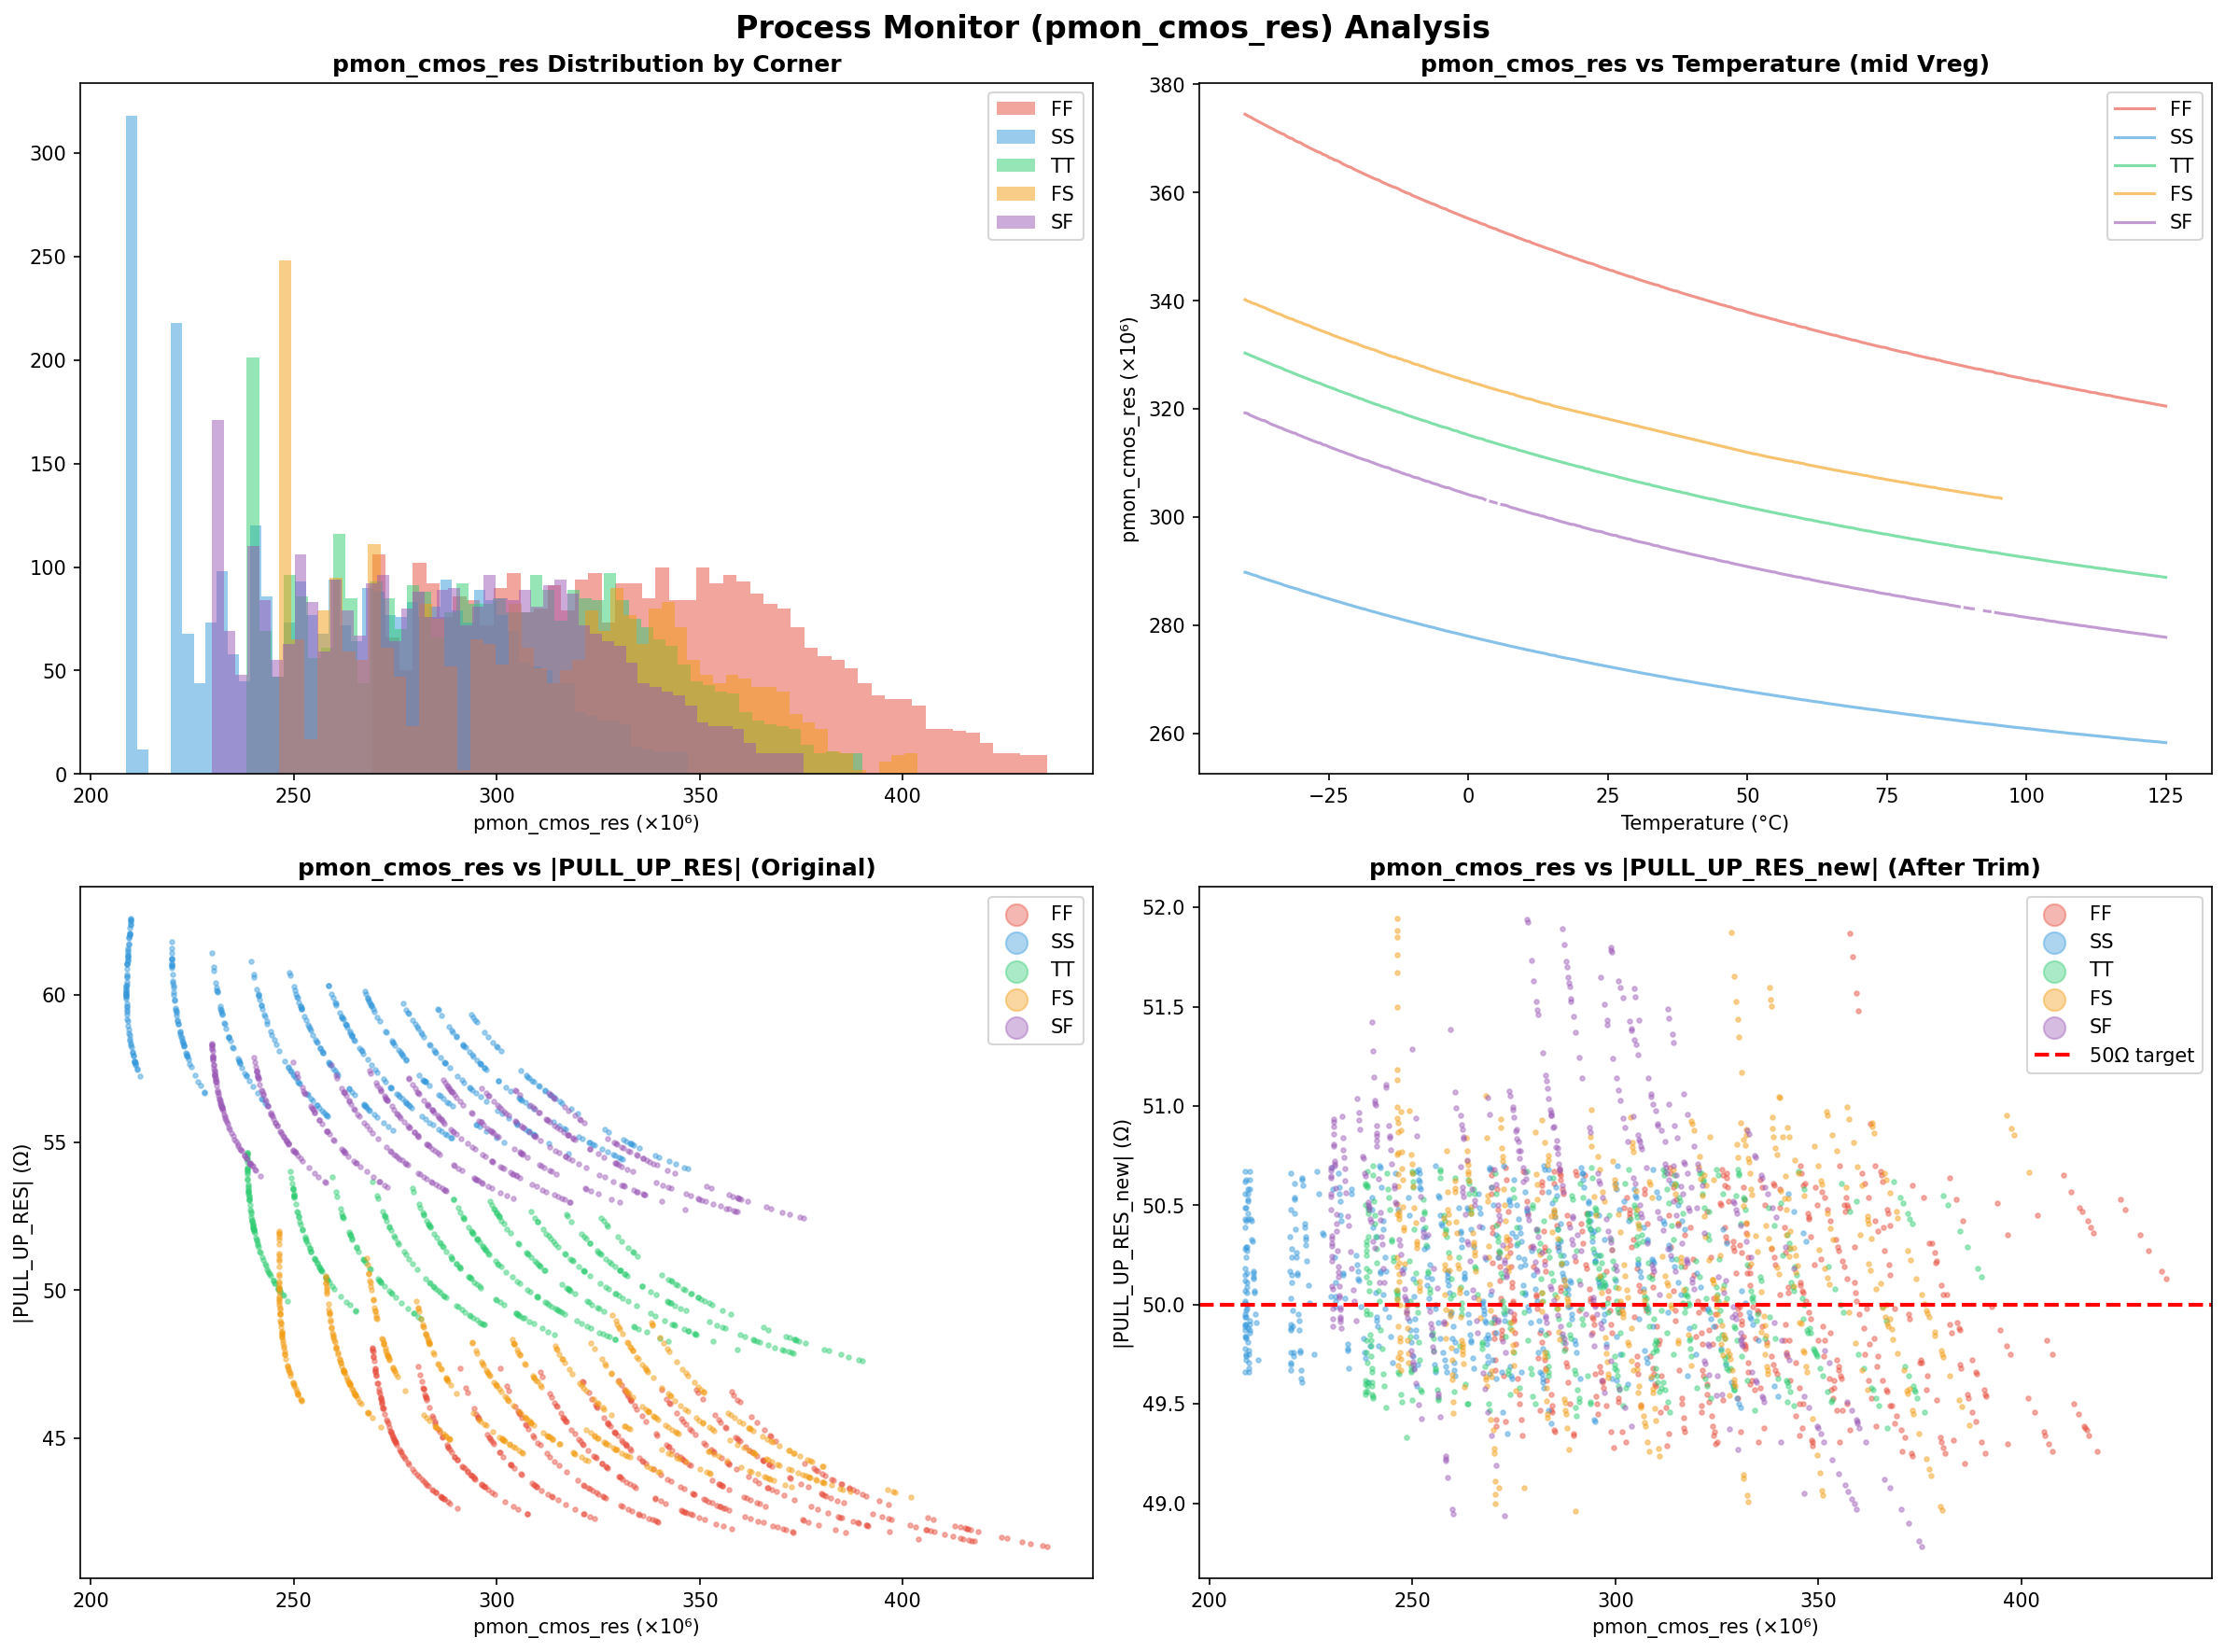
\includegraphics[width=\columnwidth]{drv_07_pmon_analysis}
\caption{Ring oscillator count (\texttt{pmon\_cmos\_res}) distributions for the 50\,$\Omega$ driver across five process corners. Significant overlap (shaded regions) makes single-input prediction impossible. Adding \texttt{vreg} and \texttt{temperature} disambiguates the overlapping cases.}
\label{fig:pmon_overlap}
\end{figure}


%% ====================================================================
%%  III. ML MODEL SELECTION
%% ====================================================================
\section{ML Model Selection}

\subsection{Model Comparison}
Five model families were evaluated for the BGR circuit (Table~\ref{tab:model_comp}). All models were trained on 80\% of data and tested on a 20\% stratified held-out set.

\begin{table}[!t]
\caption{Model Comparison for BGR Trim Prediction\label{tab:model_comp}}
\centering
\begin{tabular}{lccr}
\toprule
\textbf{Model} & \textbf{pctrl} & \textbf{nctrl} & \textbf{HW Cost} \\
\midrule
\textbf{DT (d=11/16)} & \textbf{99.57\%} & \textbf{98.88\%} & \textbf{3.88\,KB} \\
LUT (50 bins) & 99.17\% & 97.29\% & 5.96\,KB \\
Full LUT (13,860) & 100\% & 100\% & 17.3\,KB \\
Poly (deg 3) & 78.82\% & 31.64\% & 285 mult. \\
RF (10 trees, d=7) & 98.67\% & 92.93\% & 9.5\,KB \\
NN (32,16) & 98.92\% & 95.17\% & 848 mult. \\
\bottomrule
\end{tabular}
\end{table}

The DT achieves near-optimal accuracy with the smallest memory footprint and \textit{zero multipliers}. Polynomial regression fails because the trim-vs-PVT relationship is piecewise constant (staircase-shaped with discrete jumps at threshold boundaries), not smooth. Neural networks require hundreds of fixed-point multipliers, making them impractical for analog IP integration.

\begin{figure}[!t]
\centering
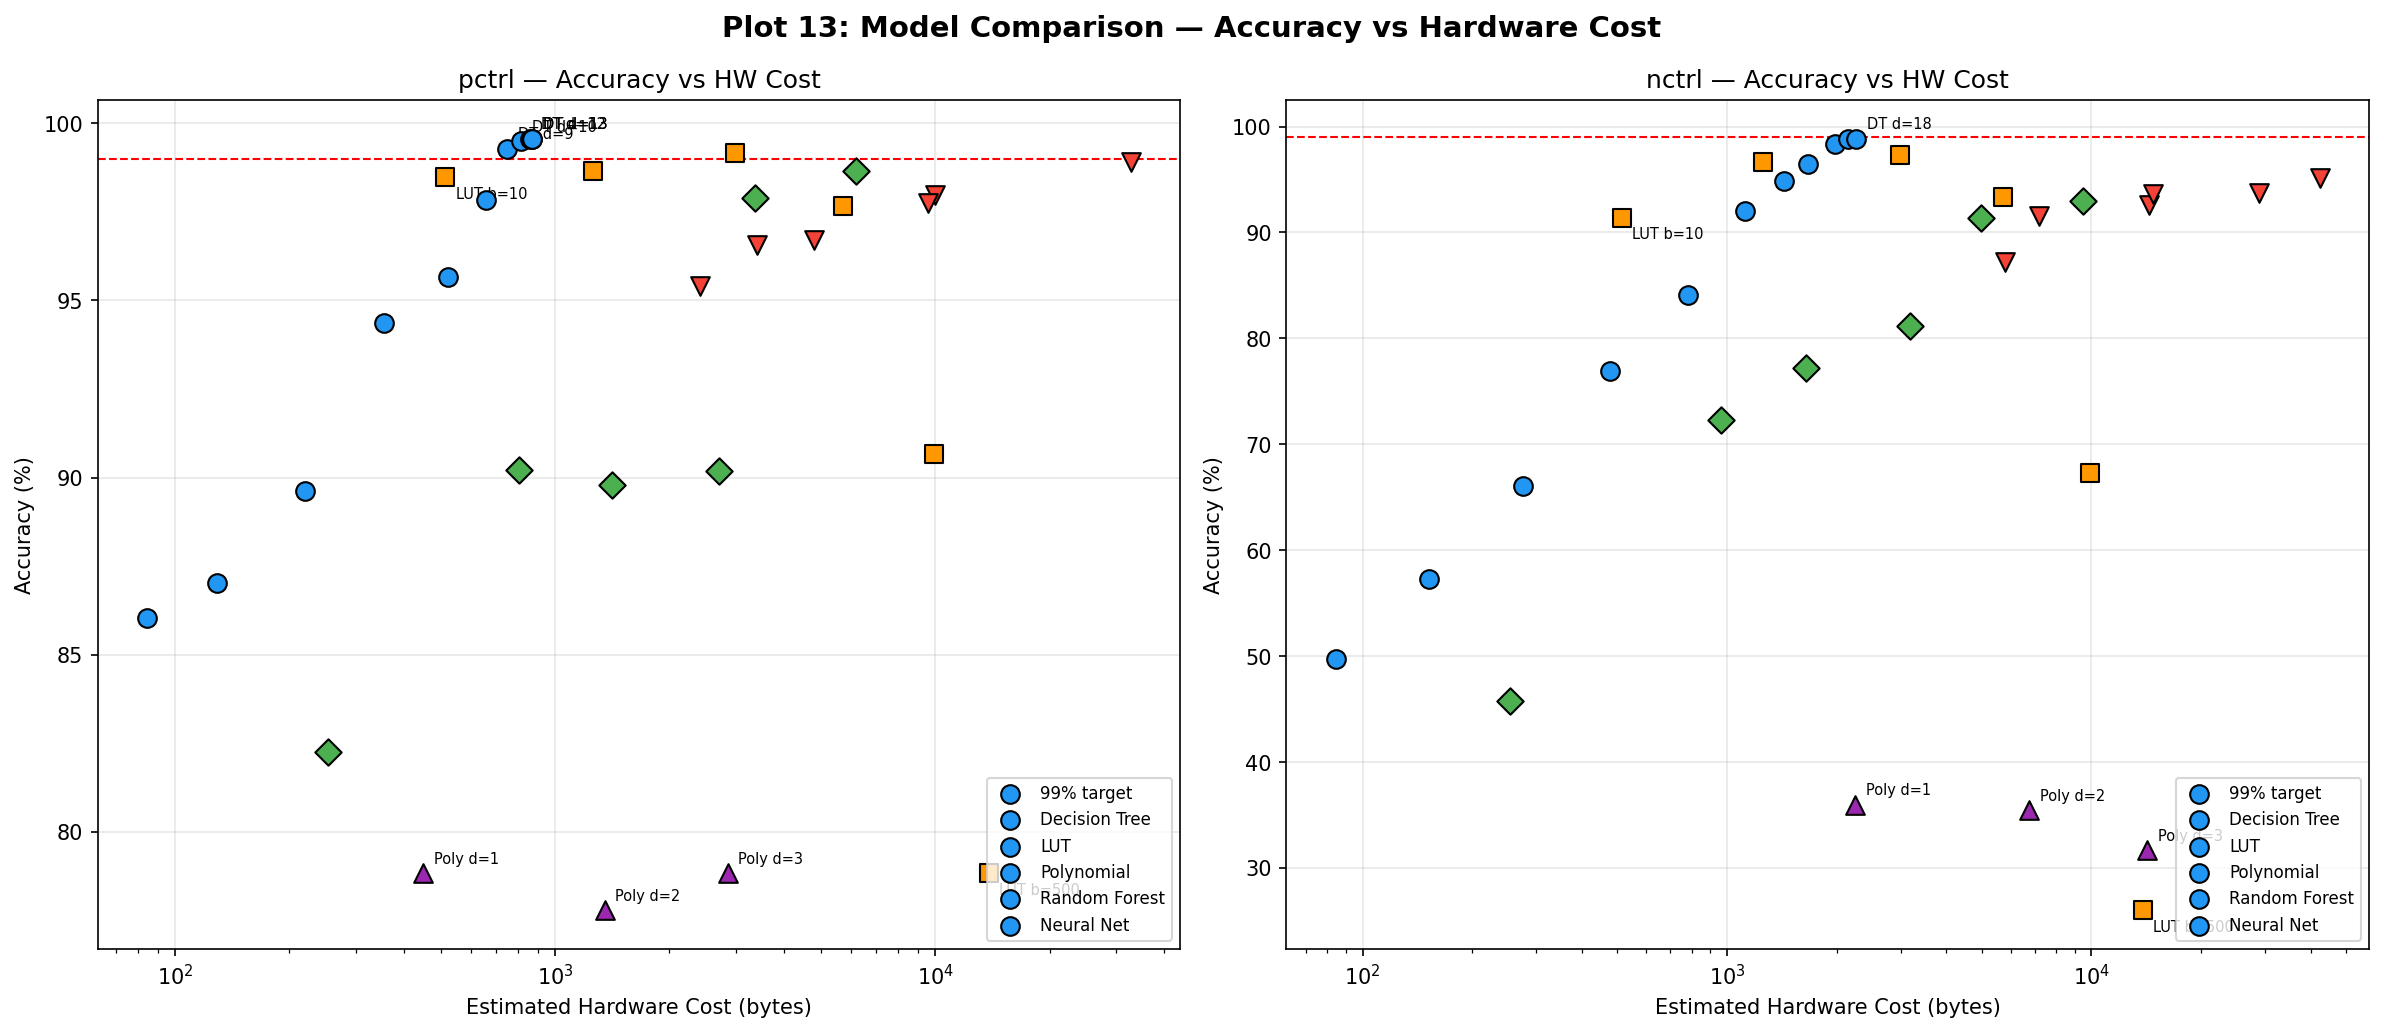
\includegraphics[width=\columnwidth]{bgr_13_model_comparison}
\caption{Accuracy vs.\ hardware cost comparison for BGR. The Decision Tree offers the best accuracy-to-cost ratio---highest accuracy with smallest memory and zero multipliers.}
\label{fig:model_comp}
\end{figure}

\subsection{Why Decision Trees Match the Physics}
The trim-vs-PVT relationship is inherently \textit{piecewise constant}: within each region of PVT space, the optimal trim code is a fixed integer that changes only when a PVT boundary is crossed. Decision Trees naturally model this behavior---each split point corresponds to a physical threshold (e.g., ``if temperature $>$ 85°C, use trim code 42; else use 38''). This is precisely why DTs outperform polynomial models, which assume smoothness.

\subsection{Depth Selection and Overfitting Analysis}
For the BGR: depths 11 (pctrl) and 16 (nctrl). For the driver: depth 14. In all cases, test accuracy \textit{increases} with depth up to the selected point, then plateaus---confirming no overfitting (Fig.~\ref{fig:depth_sweep}). Overfitting would manifest as test accuracy \textit{decreasing} beyond a certain depth.

\begin{figure}[!t]
\centering
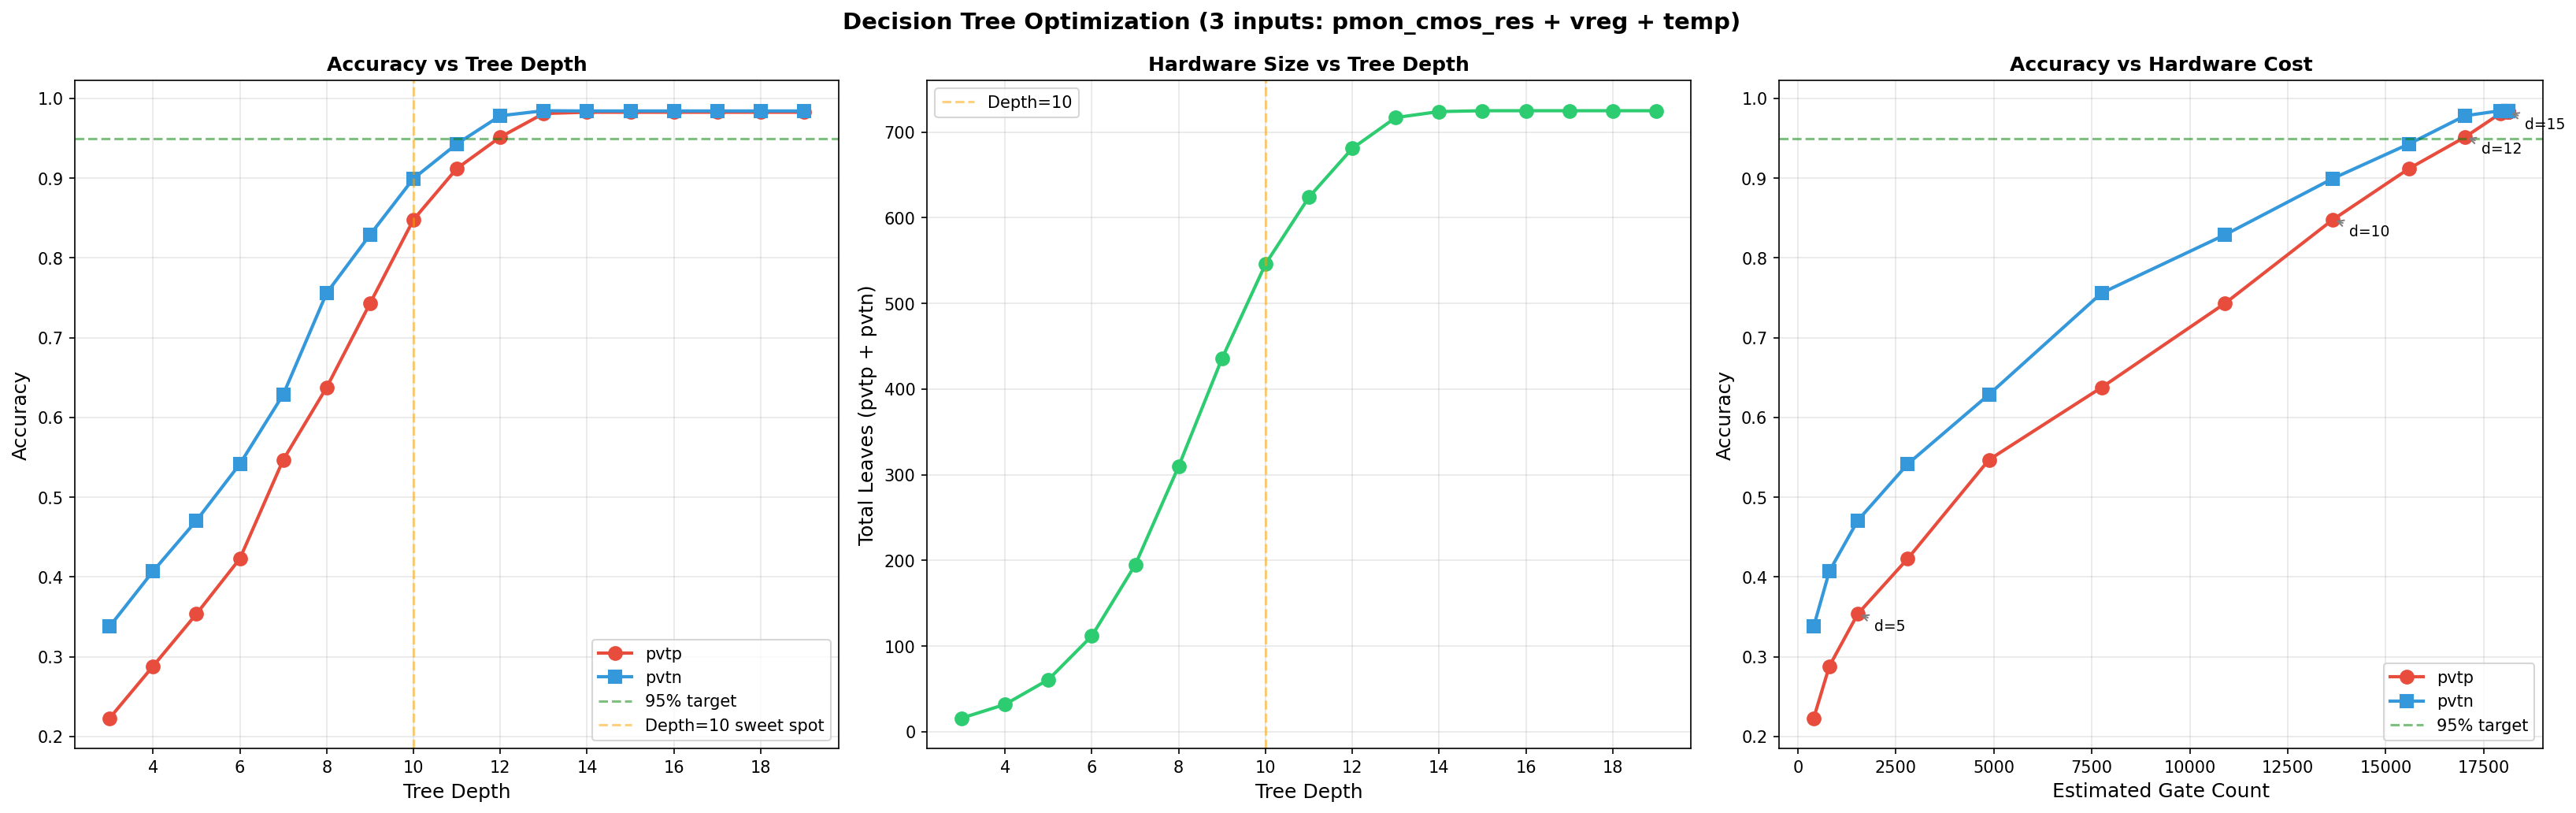
\includegraphics[width=\columnwidth]{drv_13_depth_sweep}
\caption{DT depth sweep for the 50\,$\Omega$ driver: test accuracy monotonically increases with depth up to 14, then plateaus. No sign of overfitting on the held-out test set.}
\label{fig:depth_sweep}
\end{figure}

\subsection{Feature Importance}
Gini importance analysis (Table~\ref{tab:feat_imp}) confirms all three features contribute significantly, validating the 3-input design. Notably, \texttt{vreg} has near-zero \textit{linear correlation} with trim codes ($-$0.001) but 28--30\% \textit{Gini importance}---the relationship is non-linear and conditional, which DTs capture but correlation analysis misses.

\begin{table}[!t]
\caption{Feature Importance (\%) by Gini Criterion\label{tab:feat_imp}}
\centering
\begin{tabular}{lcccc}
\toprule
& \multicolumn{2}{c}{\textbf{BGR}} & \multicolumn{2}{c}{\textbf{Driver}} \\
\cmidrule(lr){2-3} \cmidrule(lr){4-5}
\textbf{Feature} & pctrl & nctrl & pvtp & pvtn \\
\midrule
pmon\_cmos\_res & 48.2 & 47.2 & 43.5 & 46.9 \\
vreg & 28.5 & 26.5 & 30.1 & 25.8 \\
temperature & 23.3 & 26.4 & 26.4 & 27.3 \\
\bottomrule
\end{tabular}
\end{table}


%% ====================================================================
%%  IV. PROPOSED ARCHITECTURE
%% ====================================================================
\section{Proposed RTL Architecture}

\subsection{System Overview}
Fig.~\ref{fig:arch} shows the proposed architecture. Two instances of a parameterized \texttt{tree\_traversal\_fsm} module run in parallel---one per output (e.g., pctrl and nctrl for BGR). Both share input latches and start signal. Total prediction latency is $\max(d_1, d_2)$ tree depths $\times$ 2 cycles.

\begin{figure}[!t]
\centering
% TODO: Replace with actual architecture block diagram for Overleaf
\setlength{\unitlength}{1mm}
\begin{picture}(85,45)
\put(0,25){\framebox(20,18){\shortstack{\footnotesize PVT\\[-1pt]\footnotesize Sensors\\[-1pt]\footnotesize (3 inputs)}}}
\put(20,34){\vector(1,0){8}}
\put(28,30){\framebox(35,18){\shortstack{\footnotesize DT Trim Predictor\\[-1pt]\footnotesize (Top Module)}}}
\put(30,33){\framebox(14,12){\shortstack{\tiny FSM 1\\[-1pt]\tiny (Tree A)}}}
\put(47,33){\framebox(14,12){\shortstack{\tiny FSM 2\\[-1pt]\tiny (Tree B)}}}
\put(63,40){\vector(1,0){10}}
\put(63,36){\vector(1,0){10}}
\put(73,32){\framebox(12,14){\shortstack{\footnotesize Analog\\[-1pt]\footnotesize Circuit}}}
\put(74,42){\footnotesize trim1}
\put(74,34){\footnotesize trim2}
\end{picture}
\caption{System architecture: two parallel FSM instances traverse independent DT models. The same RTL module is reused for both BGR and driver circuits with parameter changes only.}
\label{fig:arch}
\end{figure}

\subsection{FSM-Based Tree Traversal}
Instead of instantiating one comparator per DT node (combinational explosion), we use a serialized 3-state FSM that reuses a single comparator:

\begin{enumerate}
\item \textbf{IDLE}: Latch inputs; set read address to root node (addr\,$=$\,0).
\item \textbf{FETCH}: Read current node data from ROM (1-cycle latency).
\item \textbf{COMPARE}: If leaf node $\rightarrow$ output trim code, assert \texttt{done}. Else $\rightarrow$ select input feature via 3:1 MUX, compare against threshold, branch to left/right child, go to FETCH.
\end{enumerate}

Each FETCH$+$COMPARE takes 2 clock cycles. Worst case: $2 \times d_{\max}$ cycles. Average latency is significantly lower since most tree paths terminate before maximum depth.

\subsection{ROM Node Encoding}
Each DT node is encoded as a fixed-width word (Table~\ref{tab:sram_format}). The 29-bit threshold width accommodates the largest input (\texttt{pmon}); smaller inputs are zero-extended for comparison.

\begin{table}[!t]
\caption{ROM Node Format\label{tab:sram_format}}
\centering
\begin{tabular}{lccl}
\toprule
\textbf{Field} & \textbf{BGR} & \textbf{Driver} & \textbf{Purpose} \\
\midrule
is\_leaf & 1\,b & 1\,b & Leaf flag \\
feat\_id & 2\,b & 2\,b & Feature select \\
threshold & 29\,b & 29\,b & Comparison value \\
left\_child & 10\,b & 10\,b & Left child addr \\
right\_child & 10\,b & 10\,b & Right child addr \\
leaf\_value & 6\,b & 8\,b & Trim code output \\
\midrule
\textbf{Total} & \textbf{58\,b} & \textbf{60\,b} & \\
\bottomrule
\end{tabular}
\end{table}


%% ====================================================================
%%  V. VALIDATION METHODOLOGY
%% ====================================================================
\section{Proof-of-Concept Validation}

Fig.~\ref{fig:validation_flow} illustrates the end-to-end validation methodology. This paper reports results for Stages~1--2 (completed); Stages~3--5 are planned for subsequent work.

\begin{figure}[!t]
\centering
\setlength{\unitlength}{1mm}
\begin{picture}(85,62)
% Stage 1
\put(5,53){\framebox(30,8){\shortstack{\footnotesize \textbf{Stage 1}\\[-1pt]\footnotesize Cadence PVT Sim}}}
\put(36,57){\makebox(10,0){\footnotesize $\checkmark$ Done}}
\put(20,53){\vector(0,-1){5}}
% Stage 2
\put(0,40){\framebox(40,8){\shortstack{\footnotesize \textbf{Stage 2}: ML Train $\rightarrow$\\[-1pt]\footnotesize RTL Verify (iverilog)}}}
\put(41,44){\makebox(10,0){\footnotesize $\checkmark$ Done}}
\put(20,40){\vector(0,-1){5}}
% Stage 3
\put(0,27){\framebox(40,8){\shortstack{\footnotesize \textbf{Stage 3}: Cadence $\leftrightarrow$\\[-1pt]\footnotesize RTL Closed-Loop}}}
\put(41,31){\makebox(15,0){\footnotesize Planned}}
\put(20,27){\vector(0,-1){5}}
% Stage 4
\put(0,14){\framebox(40,8){\shortstack{\footnotesize \textbf{Stage 4}: FPGA PoC\\[-1pt]\footnotesize (Vitis + AXI-Lite)}}}
\put(41,18){\makebox(15,0){\footnotesize Planned}}
\put(20,14){\vector(0,-1){5}}
% Stage 5
\put(0,1){\framebox(40,8){\shortstack{\footnotesize \textbf{Stage 5}: Innovus\\[-1pt]\footnotesize ASIC Synthesis}}}
\put(41,5){\makebox(15,0){\footnotesize Planned}}
\end{picture}
\caption{End-to-end validation flow. Stages 1--2 are completed and reported in this brief. Stages 3--5 are planned for follow-up work.}
\label{fig:validation_flow}
\end{figure}

\subsection{Stage 1: Cadence PVT Simulation (Completed)}
Circuit-level simulations across all PVT corners generate training data containing sensor readings and corresponding optimal trim codes. For the BGR: 13,860 samples across 3 corners. For the driver: 82,250 samples across 5 corners.

\subsection{Stage 2: ML Training and RTL Verification (Completed)}
DT models are trained using scikit-learn~\cite{sklearn} with 80/20 stratified train-test splits. The trained trees are exported as HEX files and loaded into synthesizable Verilog RTL. Functional verification is performed using Icarus Verilog~\cite{icarus} with 200 held-out test vectors per circuit.

\textbf{RTL verification results} (Table~\ref{tab:rtl_results}) confirm near-perfect functional parity between the Python-trained model and the Verilog implementation.

\begin{table}[!t]
\caption{RTL Simulation Results (200 Test Vectors Each)\label{tab:rtl_results}}
\centering
\begin{tabular}{lcc}
\toprule
\textbf{Metric} & \textbf{BGR} & \textbf{50\,$\Omega$ Driver} \\
\midrule
Output 1 accuracy & 100\% (pctrl) & 100\% (pvtp) \\
Output 2 accuracy & 99\% (nctrl) & 100\% (pvtn) \\
Combined accuracy & 99\% & 100\% \\
Avg. cycles/prediction & 18 & 22 \\
\bottomrule
\end{tabular}
\end{table}

The single nctrl mismatch in BGR is a boundary case where two adjacent trim codes produce nearly identical output voltage ($<$0.5\,mV difference). The 100\% parity for the driver confirms exact RTL-to-Python matching.

\subsection{Stage 3: Cadence$\leftrightarrow$RTL Closed-Loop (Planned)}
\textit{In progress.} The DT predictions from RTL will be fed back into the Cadence schematic to verify that the predicted trim codes actually produce the target output (0.60\,V for BGR, 50\,$\Omega$ for driver). This closes the loop between the ML model and the physical circuit behavior, providing circuit-level validation beyond functional RTL correctness.

\subsection{Stage 4: FPGA Prototyping (Planned)}
\textit{Planned.} The synthesizable RTL will be implemented on an FPGA (Xilinx) using Vitis with AXI-Lite interconnect between the Processing System (PS) and Programmable Logic (PL). The PS will supply sensor inputs and read back predicted trim codes. Key metrics to be reported:

\begin{itemize}
\item FPGA resource utilization: LUTs, flip-flops, BRAM slices consumed
\item Maximum operating frequency
\item Total on-chip power
\item Real-time prediction latency measured on hardware
\end{itemize}

\subsection{Stage 5: ASIC Synthesis (Planned)}
\textit{Planned.} Logic synthesis using Cadence Innovus with TSMC 28\,nm standard cell libraries will provide:

\begin{itemize}
\item Total gate count and silicon area (mm$^2$)
\item Critical path timing and maximum frequency
\item Dynamic and leakage power estimates
\item Comparison of synthesis results against the gate-level estimates presented in Section~\ref{sec:hw_cost}
\end{itemize}


%% ====================================================================
%%  VI. RESULTS AND COMPARISON
%% ====================================================================
\section{Results and Comparison}\label{sec:results}

\subsection{ML Accuracy Across Circuits}
Table~\ref{tab:ml_results} summarizes the ML model accuracy on held-out test data.

\begin{table}[!t]
\caption{ML Model Accuracy (Held-Out 20\% Test Set)\label{tab:ml_results}}
\centering
\begin{tabular}{lcccc}
\toprule
& \multicolumn{2}{c}{\textbf{BGR}} & \multicolumn{2}{c}{\textbf{50\,$\Omega$ Driver}} \\
\cmidrule(lr){2-3} \cmidrule(lr){4-5}
& pctrl & nctrl & pvtp & pvtn \\
\midrule
Test Accuracy & 99.57\% & 98.88\% & 98.2\% & 98.6\% \\
DT Depth & 11 & 16 & 14 & 14 \\
Total Nodes & 151 & 397 & 789 & 653 \\
\bottomrule
\end{tabular}
\end{table}

For the driver, per-corner accuracies range from 96.8\% (TT, which occupies the overlapping center of PVT space) to 99.4\% (SF/FS corners), with prediction errors almost always limited to $\pm$1 trim code ($\pm$0.2\,$\Omega$).

\subsection{Impedance After ML-Predicted Compensation}
Table~\ref{tab:impedance} demonstrates that the ML-predicted trim codes bring resistance within 0.007--0.367\,$\Omega$ of the 50\,$\Omega$ target---well within the $\pm$3\% industry specification.

\begin{table}[!t]
\caption{50\,$\Omega$ Driver: Resistance After ML Compensation\label{tab:impedance}}
\centering
\begin{tabular}{lcc}
\toprule
\textbf{Corner} & \textbf{Pull-Up R (mean)} & \textbf{Error} \\
\midrule
FF & 50.007\,$\Omega$ & 0.007\,$\Omega$ (0.01\%) \\
SS & 50.123\,$\Omega$ & 0.123\,$\Omega$ (0.25\%) \\
TT & 50.068\,$\Omega$ & 0.068\,$\Omega$ (0.14\%) \\
FS & 50.202\,$\Omega$ & 0.202\,$\Omega$ (0.40\%) \\
SF & 50.367\,$\Omega$ & 0.367\,$\Omega$ (0.73\%) \\
\bottomrule
\end{tabular}
\end{table}

\begin{figure}[!t]
\centering
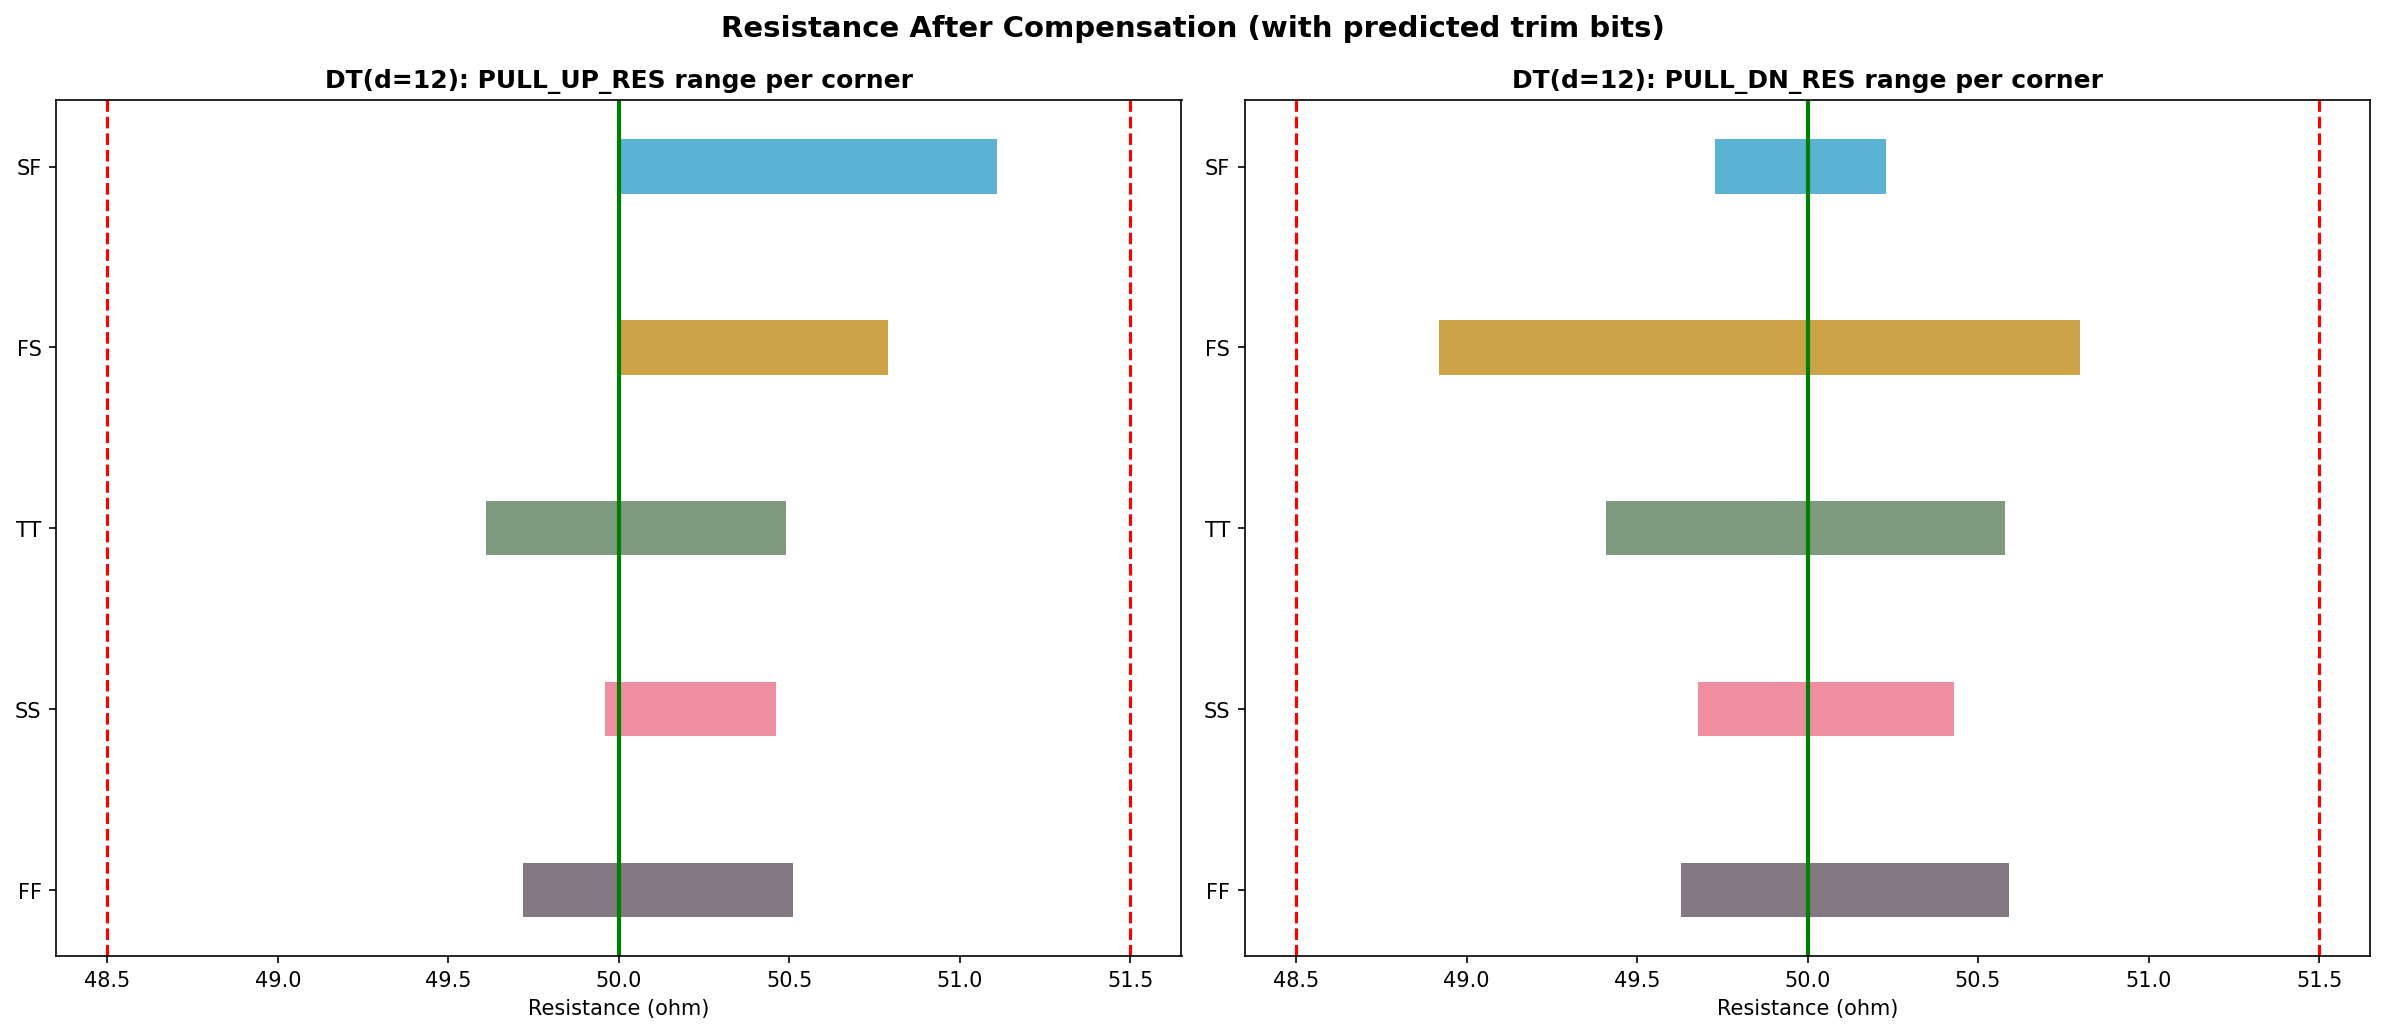
\includegraphics[width=\columnwidth]{drv_16_resistance_after_comp}
\caption{Resistance after ML-predicted trim compensation for the 50\,$\Omega$ driver. All corners fall within the $\pm$3\% specification window around 50\,$\Omega$.}
\label{fig:resistance_comp}
\end{figure}

\subsection{Hardware Cost Comparison}\label{sec:hw_cost}
Table~\ref{tab:hw_cost} provides a quantitative comparison of the proposed approach against traditional methods.

\begin{table}[!t]
\caption{Hardware Cost: Proposed vs.\ Traditional Methods\label{tab:hw_cost}}
\centering
\begin{tabular}{lccccc}
\toprule
\textbf{Method} & \textbf{Mem.} & \textbf{Lat.} & \textbf{Mult.} & \textbf{Pins} & \textbf{BOM} \\
\midrule
\multicolumn{6}{l}{\textit{BGR Circuit}} \\
\quad \textbf{DT FSM (ours)} & \textbf{3.9\,KB} & \textbf{18\,cyc} & \textbf{0} & \textbf{0} & \textbf{\$0} \\
\quad Full LUT & 17.3\,KB & 1\,cyc & 0 & 0 & \$0 \\
\quad SAR loop & $\sim$0 & 100+ & 0 & 0 & \$0 \\
\quad Poly reg. & $\sim$0 & $\sim$20 & 45+ & 0 & \$0 \\
\midrule
\multicolumn{6}{l}{\textit{50\,$\Omega$ Driver}} \\
\quad \textbf{DT FSM (ours)} & \textbf{10.6\,KB} & \textbf{22\,cyc} & \textbf{0} & \textbf{0} & \textbf{\$0} \\
\quad Ext. resistor & 0 & 100+ & 0 & 1 & \$0.05+ \\
\quad Fixed LUT & $>$20\,KB & 1\,cyc & 0 & 0 & \$0 \\
\quad NN (32,16) & $\sim$2\,KB & $\sim$10 & 848 & 0 & \$0 \\
\bottomrule
\end{tabular}
\end{table}

\subsection{Why the Proposed Approach is Better}
The advantages over traditional calibration methods are:

\begin{enumerate}
\item \textbf{Zero external components}: No precision resistors on PCB, no dedicated IC pins. Traditional external-resistor calibration costs \$0.03--0.15 per unit in BOM and consumes valuable package pin space.

\item \textbf{Zero multipliers}: The entire inference engine uses only comparisons ($\leq$), requiring $\sim$100 gates per comparator vs.\ $\sim$3,000 gates per 29-bit multiplier needed by NN approaches.

\item \textbf{$>$5$\times$ faster than SAR loops}: DT prediction completes in 18--22 cycles vs.\ 100--1000 cycles for successive approximation loops.

\item \textbf{4--5$\times$ less memory than full LUT}: The DT model compresses the PVT-to-trim mapping into a compact tree structure (3.88\,KB vs.\ 17.3\,KB for BGR; 10.6\,KB vs.\ $>$20\,KB for driver).

\item \textbf{Purely digital implementation}: No analog comparators or bias circuits needed. The design is easily portable across technology nodes---only the DT model (threshold values) changes, not the logic.

\item \textbf{Novel approach}: To our knowledge, this is the first work to demonstrate DT-based trim prediction with FSM serialization for analog calibration, validated on multiple circuit types with a complete ML-to-RTL pipeline.
\end{enumerate}

\subsection{Estimated Gate Count}
Table~\ref{tab:gates} provides a pre-synthesis estimate of the digital logic. Post-synthesis results from Innovus will be reported in follow-up work.

\begin{table}[!t]
\caption{Estimated Logic Complexity (Pre-Synthesis)\label{tab:gates}}
\centering
\begin{tabular}{lcc}
\toprule
\textbf{Component} & \textbf{BGR} & \textbf{Driver} \\
\midrule
29-bit comparators ($\times$2) & 200 & 200 \\
3:1 MUX, 29-bit ($\times$2) & 180 & 180 \\
FSM + control ($\times$2) & 150 & 150 \\
Input latches (43--44 bit) & 280 & 280 \\
Addr/depth counters ($\times$2) & 90 & 90 \\
Done synchronization & 20 & 20 \\
\midrule
\textbf{Logic total} & \textbf{$\sim$920} & \textbf{$\sim$920} \\
\textbf{ROM (28\,nm)} & 3.88\,KB & 10.56\,KB \\
\textbf{ROM area est.} & $\sim$0.005\,mm$^2$ & $\sim$0.015\,mm$^2$ \\
\bottomrule
\end{tabular}
\end{table}

\subsection{Cross-Circuit Reusability}
The same \texttt{tree\_traversal\_fsm.v} RTL module is instantiated in both circuit designs with only parameter changes (ROM depth, leaf value width). This demonstrates that the architecture is a \textit{reusable IP block} applicable to any analog circuit requiring PVT trim calibration.


%% ====================================================================
%%  VII. CONCLUSION
%% ====================================================================
\section{Conclusion}
This brief presented a hardware-efficient Decision Tree inference engine for ML-based analog trim calibration across PVT variations. The serialized FSM architecture achieves $>$98\% prediction accuracy with zero multipliers and $<$11\,KB ROM, validated on two distinct analog circuits (BGR and 50\,$\Omega$ driver) in TSMC 28\,nm CMOS. The proof-of-concept pipeline from Cadence simulation to verified RTL is complete, with FPGA prototyping (Vitis), Cadence closed-loop validation, and ASIC synthesis (Innovus) planned as next steps toward eventual silicon implementation.

Future work will extend the validation to:
\begin{itemize}
\item A third analog circuit case study to further demonstrate generalizability
\item FPGA implementation with resource utilization metrics
\item ASIC synthesis with gate count, area, power, and timing results
\item Closed-loop Cadence verification confirming circuit-level correctness
\end{itemize}


%% ====================================================================
\section*{Acknowledgments}
The authors thank the Center for VLSI and Embedded Systems (CVEST) at IIIT Hyderabad for providing access to TSMC 28\,nm PDK and Cadence simulation infrastructure.


%% ====================================================================
%%  REFERENCES
%% ====================================================================
\begin{thebibliography}{10}
\bibliographystyle{IEEEtran}

\bibitem{razavi2001}
B. Razavi, \textit{Design of Analog CMOS Integrated Circuits}, 1st~ed. New York, NY, USA: McGraw-Hill, 2001.

\bibitem{impedance_match}
J. Kim \textit{et al.}, ``A 10-Gb/s transmitter with on-chip adaptive pre-emphasis and impedance calibration in 65-nm CMOS,'' \textit{IEEE J. Solid-State Circuits}, vol.~44, no.~6, pp.~1731--1741, Jun.~2009.

\bibitem{chen2020ml}
H. Chen, Y. Li, and H. Yang, ``Machine learning assisted calibration for analog/mixed-signal circuits,'' in \textit{Proc. IEEE/ACM Int. Conf. Comput.-Aided Design (ICCAD)}, 2020, pp.~1--6.

\bibitem{lee2021mlcalib}
J. Lee, S. Park, and K. Kim, ``Neural network-based PVT compensation for high-speed serial links,'' \textit{IEEE Trans. Circuits Syst. I, Reg. Papers}, vol.~68, no.~3, pp.~1123--1134, Mar.~2021.

\bibitem{sklearn}
F. Pedregosa \textit{et al.}, ``Scikit-learn: Machine learning in Python,'' \textit{J. Mach. Learn. Res.}, vol.~12, pp.~2825--2830, 2011.

\bibitem{icarus}
S. Williams, ``Icarus Verilog,'' [Online]. Available: http://iverilog.icarus.com

\bibitem{bgr_overview}
K. N. Leung and P. K. T. Mok, ``A sub-1-V 15-ppm/°C CMOS bandgap voltage reference without requiring low threshold voltage device,'' \textit{IEEE J. Solid-State Circuits}, vol.~37, no.~4, pp.~526--530, Apr.~2002.

\bibitem{dt_hardware}
R. Struharik and B. Novak, ``Intellectual property core implementation of decision trees,'' \textit{IET Comput. Digit. Tech.}, vol.~3, no.~3, pp.~259--269, 2009.

\bibitem{sar_calib}
S. Gondi and B. Razavi, ``Equalization and clock and data recovery techniques for 10-Gb/s CMOS serial-link receivers,'' \textit{IEEE J. Solid-State Circuits}, vol.~42, no.~9, pp.~1999--2011, Sep.~2007.

\bibitem{pvt_monitor}
K. A. Bowman \textit{et al.}, ``A 45 nm resilient microprocessor core for dynamic variation tolerance,'' \textit{IEEE J. Solid-State Circuits}, vol.~46, no.~1, pp.~194--208, Jan.~2011.

\end{thebibliography}

\vfill

\end{document}
